\documentclass[12pt,a4paper]{article}
\renewcommand{\baselinestretch}{1.05}
\usepackage[spanish]{babel}
%\usepackage[utf8]{inputenc}

\usepackage{amsmath,amsthm,verbatim,amssymb,amsfonts,amscd, graphicx}
\usepackage{graphicx}
\usepackage{caption}
\usepackage{subcaption}
\usepackage{tkz-fct}
\usetikzlibrary{babel}
\usepackage{pgfplots}
\usepackage{booktabs}
\usepackage{float}
\usepackage{enumitem}
\usepackage{forest}
\usepackage{hyperref}
\usepackage{fancybox}
\usepackage{listings}

%Uso de la fuente Source Sans Pro

\usepackage[default]{sourcesanspro}
%\usepackage[T1]{fontenc}

%Controlar la partición de palabras.
\pretolerance=5000
\tolerance=6000

%Simbolo de euro
\usepackage{eurosym} % para el euro


%Definición de monospace para codigo inline y paquete listings para código fuente.
\def\code#1{\texttt{#1}}
\usepackage{listingsutf8}
\lstset{
    %extendedchars=false,
    %inputencoding=utf8
}
\usepackage{color}
\definecolor{grisclarito}{gray}{0.95}

\lstdefinestyle{customc}{
  %belowcaptionskip=1\baselineskip,
  breaklines=true,
  frame=single,
  %xleftmargin=\parindent,
  language=C,
  showstringspaces=false,
  %basicstyle=\ttfamily,
  keywordstyle=\bfseries\color{green!40!black},
  commentstyle=\itshape\color{purple!40!black},
  identifierstyle=\color{blue},
  stringstyle=\color{orange},
  backgroundcolor=\color{grisclarito}
}

\hypersetup{
  colorlinks=true,
  linkcolor=black,
  urlcolor=blue
}

\setcounter{secnumdepth}{5}

\setlength{\parindent}{0pt}
\topmargin0.0cm
\headheight0.0cm
\headsep0.0cm
\oddsidemargin0.0cm
\textheight23.0cm
\textwidth16.5cm
\footskip1.0cm

\renewcommand*\contentsname{Índice}
\newcommand{\mylabel}[2]{#2\def\@currentlabel{#2}\label{#1}}

\begin{document}
\begin{titlepage}
  \centering
  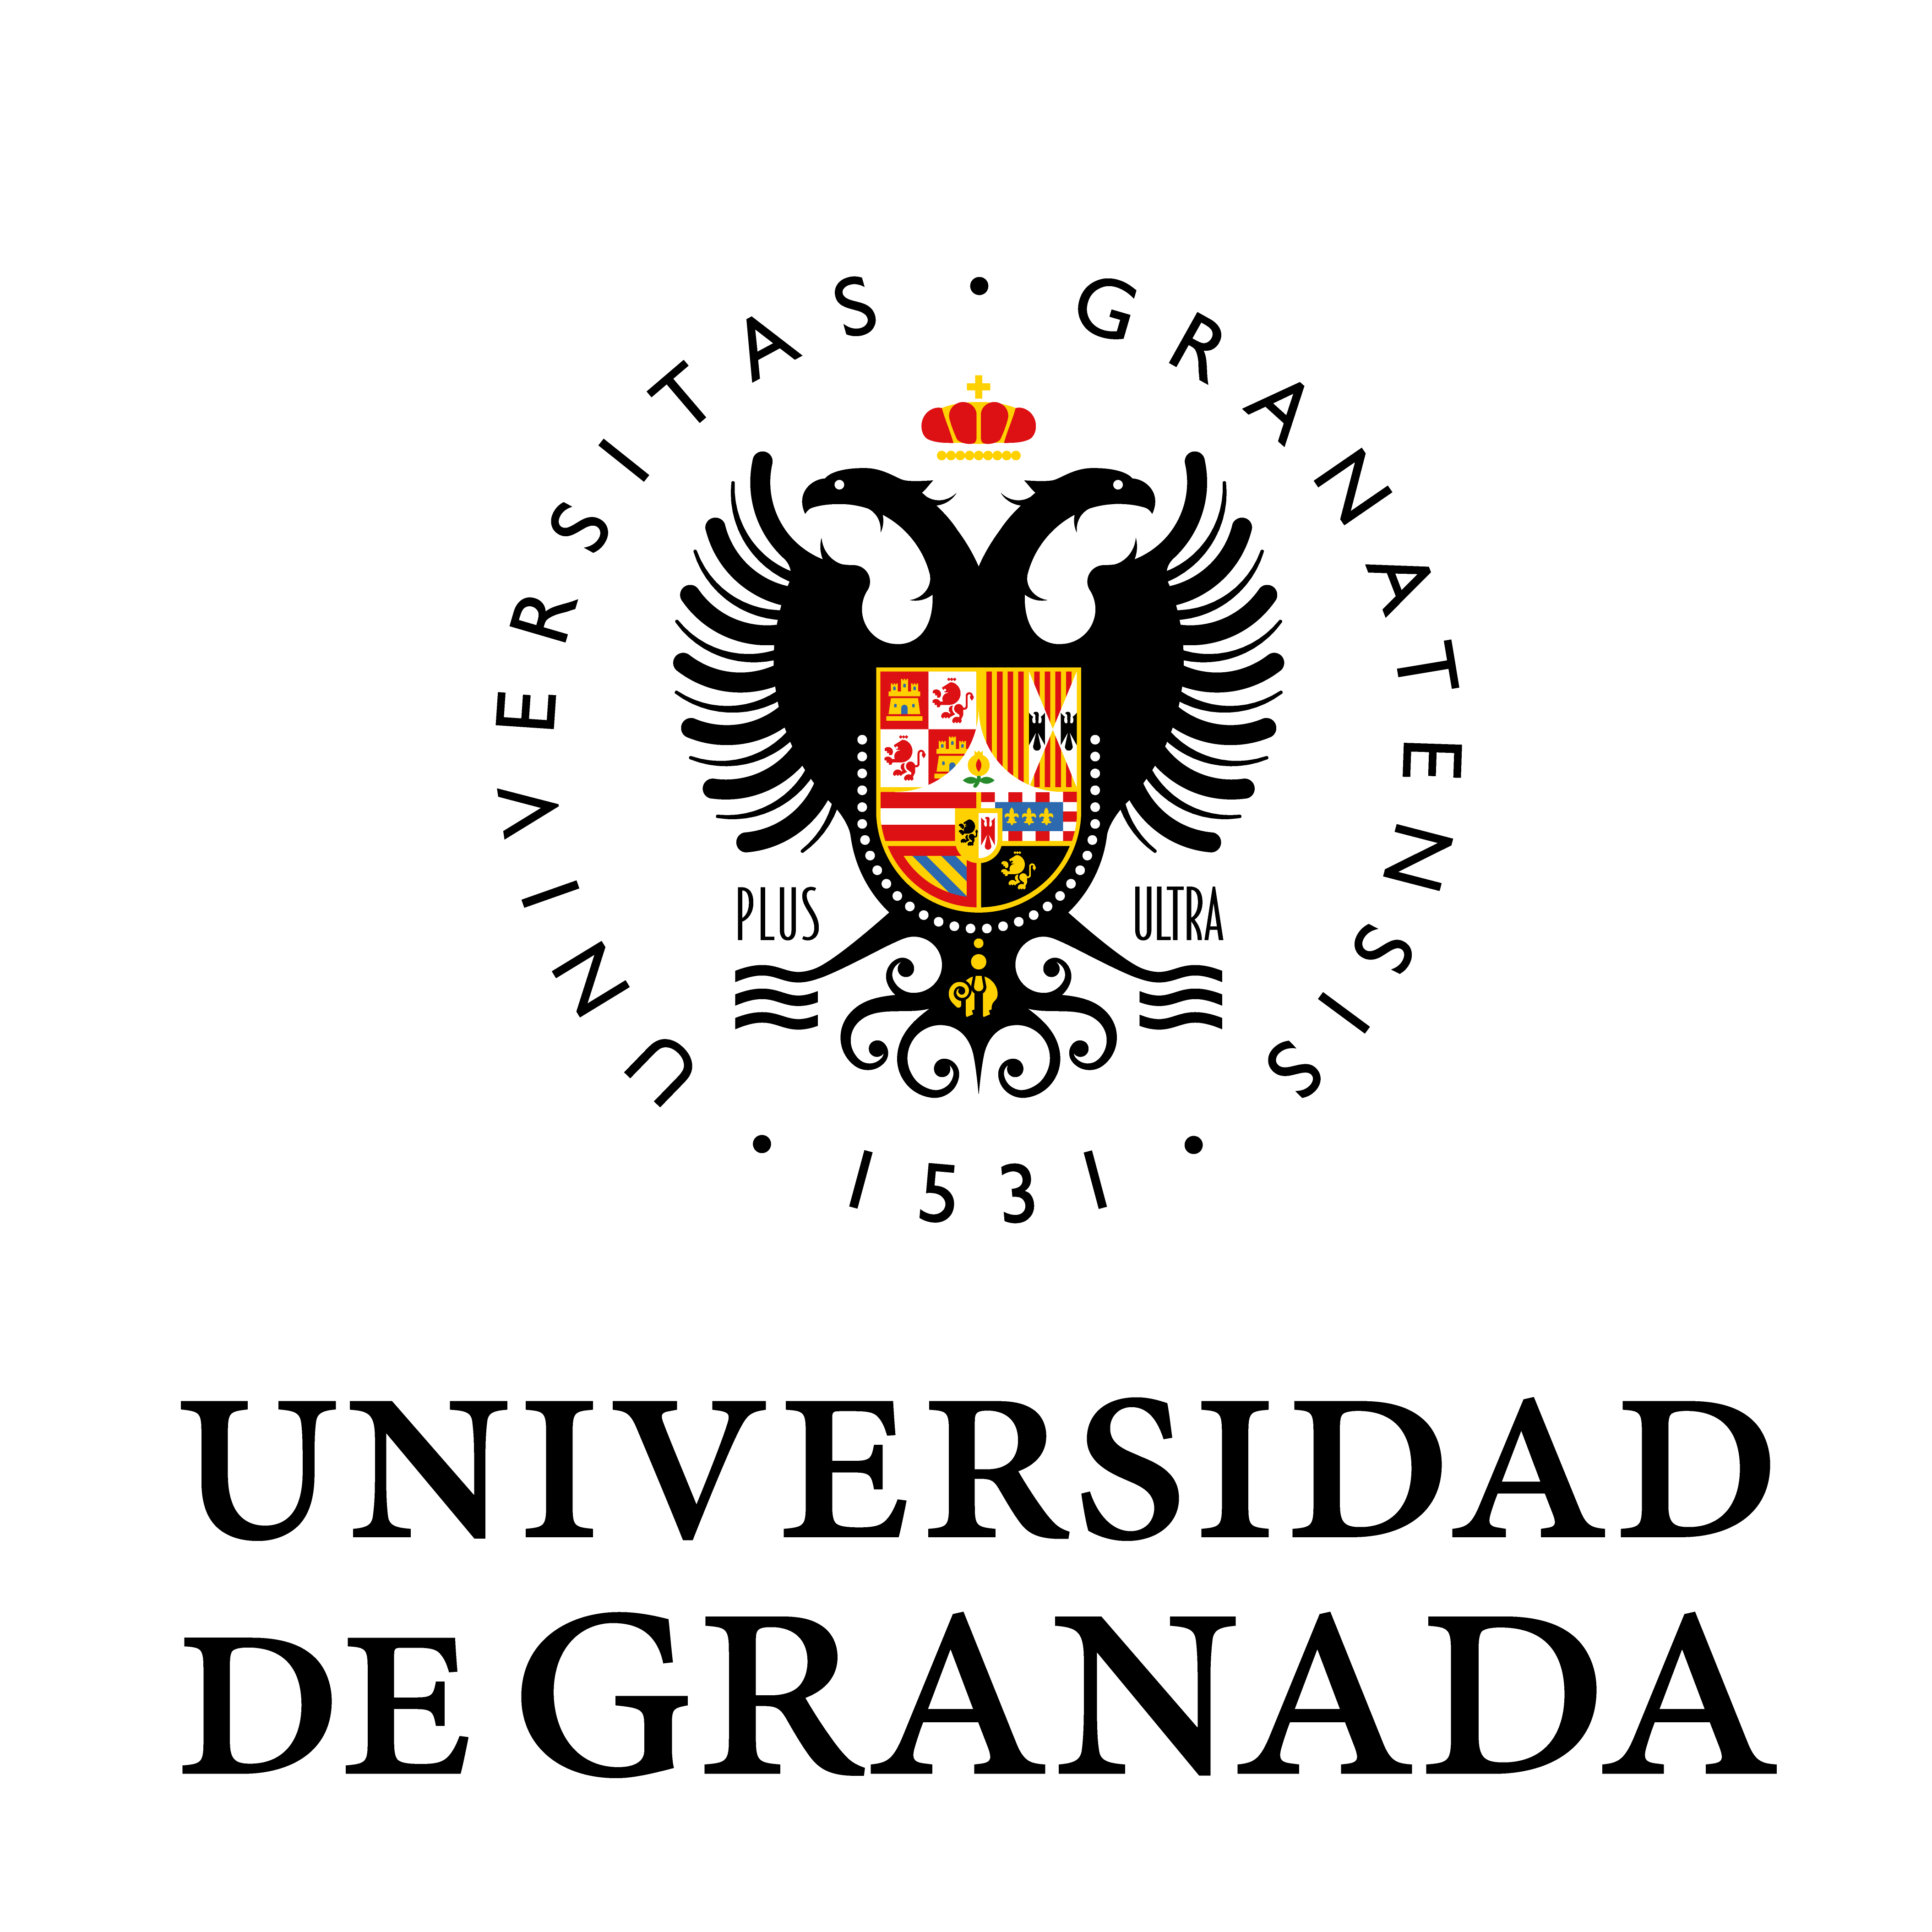
\includegraphics[width=0.6\textwidth]{imagenes/ugr.png}\par\vspace{1cm}
  {\scshape\large Diseño y Desarrollo de Sistemas de Información \par} \vspace{1cm}
  {\huge\bfseries Diseño de un sistema de información para la gestión y reproducción de música. \par}
  \vspace{0.4cm}
  {\large\itshape Entrega final.}
  \vspace{0.6cm}
  {\large\itshape \\ Darío Abad Tarifa \\ Juan Francisco Díaz Moreno \\ Pedro Domínguez López \\ Javier Sáez de la Coba \par} \vspace{1.00cm}
  Curso 2018-2019 \\
  \vfill

  % Bottom of the page
  {\large \today\par}
\end{titlepage}

\tableofcontents
\newpage

\setlength{\parskip}{10pt}

\section{Descripción del problema a resolver.}

Una empresa de streaming de audio quiere rehacer su plataforma de gestión de música (todo el servicio excepto el propio streaming de música). Para ello requiere que puedan haber cuentas de oyentes y de artistas.

El sistema ofrece un servicio de musica en streaming, es decir permite que un usuario pueda buscar una cancion, un album o una lista de musica en la base 
de datos para posteriormente escucharla. 

Las listas funcionan como si de un directorio se tratase, el usuario las gestiona como quiere y en ellas guarda sus canciones favoritas o canciones segun un tema especifico.  

El sistema ofrece ademas diferentes opciones de carácter social para facilitar la relación entre amigos y los artistas con sus oyentes. Un usuario puede seguir a otro usuario (sea artista o no) para estar al corriente de lo que escucha proporcionando el nombre del usuario al que quiere seguir. Un usuario podrá recomendar una canción a otro usuario proporcionando el nombre de este y el identificador de la canción que quiere recomendar. Un usuario podrá solicitar un resumen sobre las canciones que escucha su lista de amigos. 
Un usuario podrá ver las recomendaciones que le llegan de sus amigos. Además, los usuarios oyentes pueden valorar las canciones que escuchan. Por último podrán visualizar las canciones mejor valoradas por un usuario proporcionando su nombre de usuario.P

\section{Análisis de requisitos.}

\subsection{Requisitos de datos}

\begin{enumerate}[label=\textnormal{RD\arabic*.}]

	\item Identificador de la canción, álbum o lista para escuchar: \label{rd1}
		\begin{itemize}
			\item Elección (canción, álbum o lista)
			\item Identificador
		\end{itemize}
		
	\item Datos de álbum almacenado: \label{rd2}
		\begin{itemize}
			\item Nombre del álbum
			\item Nombre del artista
			\item Fecha de introducción
			\item Identificador del álbum
        	\item Nombre del álbum
		    \item Nombre del artista
		    \item Fecha de introducción
			\item Número de canciones
			\item Duración
		\end{itemize}
		
		
	\item Datos de canción almacenada: \label{rd3}
		\begin{itemize}
			\item Identificador de la canción
		    \item Nombre de la canción
		    \item Nombre del artista
		    \item Nombre del álbum
		    \item Estilo de la canción
		    \item Duración de la canción
		    \item Fecha de introducción
		    \item Archivo de audio
		    \item Número de reproducciones
		    \item Valoración media
		\end{itemize}
		
	\item Datos de lista almacenada: \label{rd4}
		\begin{itemize}
		    \item Identificador de la lista
		    \item Nombre de la lista
		    \item Canciones que contiene
		    \item Duración de la lista
		    \item Fecha de creacion
		    \item Usuario al que pertenece
		    \item Seguidores
		\end{itemize}
		
	\item Identificador de la nueva lista creada: \label{rd5}
		\begin{itemize}
			\item Identificador de la lista
		\end{itemize}
		
	\item Nombre para la busqueda de una cancion, album o lista: \label{rd6}
		\begin{itemize}
			\item Nombre
		\end{itemize}
		
	\item Lista con los posibles identificadores según el resultado de la búsqueda: \label{rd7}
		\begin{itemize}
			\item Identificador
			\item Tipo: canción, álbum, lista
			\item Nombre
			\item Usuario o artista
			\item Fecha de publicación o de creación
			\item Duracionr
		\end{itemize}
		
	\item Datos para crear una lista nueva: \label{rd8}
		\begin{itemize}
			\item Usuario
			\item Fecha 
		\end{itemize}
		
	\item Valoración de una canción: \label{rd9}
		\begin{itemize}
			\item Identificador de la canción
			\item Identificador
		\end{itemize}
		
	\item Datos nuevo álbum: \label{rd10}
		\begin{itemize}
		    \item Nombre del álbum
		    \item Nombre del artista
		    \item Fecha de introducción
		\end{itemize}
		
	\item Datos nueva canción: \label{rd11}
		\begin{itemize}
		    \item Nombre de la canción
		    \item Nombre del artista
		    \item Nombre del álbum
		    \item Estilo de la canción
		    \item Duración de la canción
		    \item Fecha de introducción
		    \item Archivo de audio
		\end{itemize}
		
	\item  Identificador de la canción introducida: \label{rd12}
		\begin{itemize}
			\item Identificador de la canción
		\end{itemize}
		
	\item Identificador de la canción para ver sus estadísticas: \label{rd13}
		\begin{itemize}
			\item Identificador de la canción
		\end{itemize}
		
	\item Reproduccion de una lista: \label{rd14}
		\begin{itemize}
		   	\item Audio de las canciones de la lista
		\end{itemize}
		
	\item Estadísticas de la canción: \label{rd15}
		\begin{itemize}
		    \item Nombre de la canción
		    \item Número de reproducciones
		    \item Valoración media
		\end{itemize}
		
	\item Identificador de la canción para añadirla a canciones destacadas: \label{rd16}
		\begin{itemize}
			\item Identificador de la canción
		\end{itemize}
		
	\item Lista de las canciones destacadas actualizada: \label{rd17}
		\begin{itemize}
			\item Canciones destacadas
		\end{itemize}
		
	\item Identificador de la canción o álbum para eliminarlo: \label{rd18}
		\begin{itemize}
			\item Elección (canción o álbum)
			\item Identificador
		\end{itemize}
		
	\item Datos de registro del usuario: \label{rd19}
		\begin{itemize}
			\item Nombre de usuario
			\item Correo electrónico
			\item Contraseña
			\item Nombre
			\item Apellidos
			\item Tipo de usuario (oyente, artista)
			\item Dirección
		\end{itemize}
		
	\item Datos usuario almacenado: \label{rd20}
		\begin{itemize}
			\item Identificador
			\item Nombre de usuario
			\item Correo electrónico
			\item Contraseña
			\item Nombre
			\item Apellidos
			\item Tipo de usuario (oyente, artista)
			\item Dirección
		\end{itemize}
		
	\item Contraseña nueva: \label{rd21}
		\begin{itemize}
			\item Identificador de usuario
			\item Contraseña nueva
		\end{itemize}
		
	\item Datos perfil usuario: \label{rd22}
		\begin{itemize}
			\item Nombre de usuario
			\item Correo electrónico
			\item Contraseña
			\item Nombre
			\item Apellidos
			\item Dirección
		\end{itemize}
		
	\item Identificador del usuario a eliminar: \label{rd23}
		\begin{itemize}
			\item Identificador del usuario
		\end{itemize}
		
		
	\item Datos de un usuario:  \label{rd24}
		\begin{itemize}
			\item Nombre de usuario
		\end{itemize}

	\item Datos de un amigo:  \label{rd25}
		\begin{itemize}
			\item Nombre de usuario
			\item Canción que está escuchando
		\end{itemize}
	\item Datos de artista  \label{rd26}
		\begin{itemize}
			\item Nombre de usuario
			\item Nombre artístico
			\item Número de canciones subidas
			\item Álbumes subidos
		\end{itemize}
	\item Recomendación saliente  \label{rd27}
		\begin{itemize}
			\item Nombre de usuario de salida
			\item Cuerpo de mensaje
			\item Nombre de usuario de entrada
		\end{itemize}
	\item Recomendación entrante  \label{rd28}
		\begin{itemize}
			\item Nombre de usuario de entrada
			\item Cuerpo de mensaje
			\item Nombre de usuario de salida
		\end{itemize}
	\item Recomendación almacenada.  \label{rd29}
		\begin{itemize}
			\item Nombre de usuario que recomienda
			\item Cuerpo de mensaje
			\item Nombre de usuario que es recomendado
		\end{itemize}
	\item Datos de canción que está siendo escuchada  \label{rd30}
		\begin{itemize}
			\item Identificador de canción
			\item Usuario que la está escuchando
		\end{itemize}
	\item Datos del usuario actual  \label{rd31}
		\begin{itemize}
			\item Identificador de usuario
		\end{itemize}
	\item Datos de canciones mejor valoradas  \label{rd32}
		\begin{itemize}
			\item Identificadores de canciones
			\item Identificador de usuario que ha valorado
		\end{itemize}
	\item Datos de usuario que ha realizado valoraciones  \label{rd33}
		\begin{itemize}
			\item Nombre de usuario
		\end{itemize}
		
	\item Valoración dada por un usuario a una canción  \label{rd34}
		\begin{itemize}
			\item identificador de canción
			\item Valoración
		\end{itemize}
		
	\item Datos modificar estado de canción en lista.  \label{rd35}
		\begin{itemize}
			\item Identificador de canción
			\item Identificador de la lista de reproducción
			\item Operación a realizar
		\end{itemize}
		
	\item Identificador de la lista a eliminar  \label{rd36}
		\begin{itemize}
			\item Identificador de la lista de reproducción
		\end{itemize}
		
	\item Datos canciones que estan siendo escuchadas  \label{rd37}
		\begin{itemize}
			\item Identificador de la cancion
			\item Identificador de usuario que escucha la cancion
		\end{itemize}
				
	\item Datos recomendaciones almacenadas  \label{rd38}
		\begin{itemize}
			\item Identificador del usuario que recomienda
			\item Identificador del usuario que recibe la recomendación
			\item Identificador de la canción que es recomendada
		\end{itemize}
		
	\item Datos canciones mejor valoradas \label{rd39}
		\begin{itemize}
			\item Nombre de la cancion
			\item Nombre del artista
			\item Valoración
		\end{itemize}

\end{enumerate}


\subsection{Requisitos funcionales}

\begin{enumerate}[label=\textnormal{RF\arabic*.}]

%%%%%%%%%%%%%%%%%% AREA FUNCIONAL ESCUCHAR CANCIONES

    \item Escuchar una canción: un usuario introduce el identificador de la canción, álbum o lista que quiere escuchar.\label{rf1}.
    	\begin{itemize}
			\item Entrada: \ref{rd1}
			\item Consulta: \ref{rd2}, \ref{rd3}, \ref{rd4} 
			\item Salida: \ref{rd14}
		\end{itemize}
		
	 \item Buscar una canción: a través del nombre de una canción, álbum o lista se elige el identificador que se considere el adecuado con los criterios de búsqueda \label{rf2}.
    	\begin{itemize}
			\item Entrada: \ref{rd6}
			\item Consulta: \ref{rd2}, \ref{rd3}, \ref{rd4} 
			\item Salida: \ref{rd7}
		\end{itemize}

	 \item Crear listas de reproducción: un usuario puede crear una lista donde añade canciones y las tiene todas en un mismo lugar. \label{rf3}.
    	\begin{itemize}
			\item Entrada: \ref{rd8}
			\item Almacena: \ref{rd4}
			\item Salida: \ref{rd5}
		\end{itemize}

	 \item Añadir canciones a una lista de reproducción: un usuario puede añadir o eliminar las canciones de su lista a traves del identificador.\label{rf4}.
    	\begin{itemize}
			\item Entrada: \ref{rd35}
			\item Consulta: \ref{rd4}
			\item Actualiza: \ref{rd4}
		\end{itemize}

	 \item Borrar lista: un usuario puede eliminar su lista.\label{rf5}.
    	\begin{itemize}
			\item Entrada: \ref{rd36}
			\item Consulta: \ref{rd4}
			\item Actualiza: \ref{rd4}
		\end{itemize}
		
	 \item Valorar canciones: un usuario puede valorar una canción.\label{rf6}.
    	\begin{itemize}
			\item Entrada: \ref{rd34}
			\item Consulta: \ref{rd9}
			\item Actualiza: \ref{rd9}
		\end{itemize}
		
%%%%%%%%%%%%%%%%%% AREA FUNCIONAL SUBIR CANCIONES
		
	 \item Crear álbum: un artista registra en el sistema un nuevo álbum.\label{rf7}.
    	\begin{itemize}
			\item Entrada: \ref{rd10}
			\item Almacena: \ref{rd2}
			\item Salida: ninguna
		\end{itemize}
		
	 \item Crear canción: un artista introduce en el sistema una nueva canción.\label{rf8}.
    	\begin{itemize}
			\item Entrada: \ref{rd11}
			\item Consulta: \ref{rd2}
			\item Actualiza: \ref{rd3}
			\item Salida: \ref{rd12} 
		\end{itemize}
		
	 \item Ver estadísticas de canción: un artista consulta las estadísticas de una de sus canciones buscándola con su identificador.\label{rf9}.
    	\begin{itemize}
			\item Entrada: \ref{rd13}
			\item Consulta: \ref{rd12}
			\item Salida: \ref{rd15}
		\end{itemize}
		
	 \item Destacar canciones individuales: un artista selecciona una canción a través de su identificador y la añade a su lista de canciones destacadas.\label{rf10}.
    	\begin{itemize}
			\item Entrada: \ref{rd16}
			\item Consulta: \ref{rd3}
			\item Salida: \ref{rd17}
		\end{itemize}
		
	 \item Borrar canciones: un artista introduce en el sistema si quiere eliminar una canción o un álbum y el identificador de su elección y el sistema elimina los datos asociados al mismo.\label{rf11}.
    	\begin{itemize}
			\item Entrada: \ref{rd18}
			\item Consulta: \ref{rd2} \ref{rd3} 
			\item Actualiza: \ref{rd2} \ref{rd3} 
		\end{itemize}
		
%%%%%%%%%%%%%%%%%%%%%%% ÁREA DE ADMINISTRACIÓN DE USUARIOS
		
	 \item Crear usuarios. El sistema guarda la información de un nuevo usuario \label{rf12}.
    	\begin{itemize}
			\item Entrada: \ref{rd19}
			\item Almacena: \ref{rd20}
		\end{itemize}
		
	 \item Recuperar contraseña: \label{rf13}.
    	\begin{itemize}
			\item Entrada: \ref{rd21}
			\item Actualiza: \ref{rd20}
		\end{itemize}
		
	 \item Modificar perfil. El sistema guarda la información modificada por el usuario. \label{rf14}.
    	\begin{itemize}
			\item Entrada: \ref{rd22}
			\item Almacena: \ref{rd20}
		\end{itemize}
		
	 \item Borrar usuarios. Eliminar a un usuario del sistema.\label{rf15}.
    	\begin{itemize}
			\item Entrada: \ref{rd23}
			\item Actualiza: \ref{rd20}
		\end{itemize}
		
%%%%%%%%%%%%%%%%%%%%%%%%% ÁREA SOCIAL
		
	 \item Seguir usuario. Se crea una relación entre dos usuarios, el seguidor estará al tanto de las acciones del usuario al que sigue. \label{rf16}
	 	\begin{itemize}
			\item Entrada: \ref{rd24}
			\item Almacenado: \ref{rd26}
		\end{itemize}
	
	 \item Recomendar canciones a amigos. Un usuario envía a través de un mensaje una canción a otro usuario. \label{rf17}
	 	\begin{itemize}
			\item Entrada: \ref{rd27}
			\item Almacenado: \ref{rd29}
		\end{itemize}
	
	 \item Ver lo que están escuchando los amigos. Se muestra al usuario una lista con las canciones que están escuchando sus amigos en ese momento. \label{rf18}
	 	\begin{itemize}
			\item Entrada: \ref{rd25}
			\item Consulta: \ref{rd37}
			\item Salida: \ref{rd30}
		\end{itemize}

	 \item Ver recomendaciones entrantes. Se muestra al usuario una lista con las recomendaciones que le han hecho sus amigos. \label{rf19}
	 	\begin{itemize}
			\item Entrada: \ref{rd31}
			\item Consulta: \ref{rd38}
			\item Salida: \ref{rd28}
		\end{itemize}

	 \item Canciones mejor valoradas por un usuario. Un usuario solicita una lista de las canciones mejor valoradas proporcionando el identificador de otro usuario. \label{rf20}
	 	\begin{itemize}
			\item Entrada:  \ref{rd33}
			\item Consulta: \ref{rd32}
			\item Salida: \ref{rd39}
		\end{itemize}	
   
\end{enumerate}


\subsection{Validación cruzada de requisitos}
\begin{table}[H]
\begin{center}
\begin{tabular}{|c|c|c|c|}
\hline
	RF & Entrada & Manejo & Salida\\
\hline
	\ref{rf1} & \ref{rd1} & \ref{rd2},\ref{rd3},\ref{rd4} & \ref{rd14}\\
\hline
	\ref{rf2} & \ref{rd6} & \ref{rd4} & \ref{rd7}\\
\hline
	\ref{rf3} & \ref{rd8} & \ref{rd4} & \ref{rd5}\\
\hline
	\ref{rf4} & \ref{rd5} & \ref{rd4} & \\
\hline
	\ref{rf5} & \ref{rd36} & \ref{rd4} & \\
\hline
	\ref{rf6} & \ref{rd5} & \ref{rd9} & \ref{rd9}\\
\hline
	\ref{rf7} & \ref{rd10} & \ref{rd2} & \\
\hline
	\ref{rf8} & \ref{rd11} & \ref{rd2},\ref{rd3} & \ref{rd12}\\
\hline
	\ref{rf9} & \ref{rd13} & \ref{rd12} & \ref{rd15}\\
\hline
	\ref{rf10} & \ref{rd16} & \ref{rd3},\ref{rd10} & \ref{rd17}\\
\hline
	\ref{rf11} & \ref{rd18} & \ref{rd2},\ref{rd3},\ref{rd10} & \\
\hline
	\ref{rf12} & \ref{rd19} & \ref{rd20} & \\
\hline
	\ref{rf13} & \ref{rd21} & \ref{rd20} & \\
\hline
	\ref{rf14} & \ref{rd22} & \ref{rd20} & \\
\hline
	\ref{rf15} & \ref{rd23} & \ref{rd20} & \\
\hline
	\ref{rf16} & \ref{rd24} & \ref{rd25},\ref{rd26} & \\
\hline
	\ref{rf17} & \ref{rd27} & \ref{rd29} & \\
\hline
	\ref{rf18} & \ref{rd25} & \ref{rd37} & \ref{rd30}\\
\hline
	\ref{rf19} & \ref{rd31} & \ref{rd38} & \ref{rd28}\\
\hline
	\ref{rf20} & \ref{rd33} & \ref{rd32} & \ref{rd39}\\
\hline
\end{tabular}
\end{center}
\caption{Requisitos funcionales}
\end{table}

\begin{table}[H]
\begin{center}
\begin{tabular}{|c|c|c|c|}
\hline
	RD & Entrada & Manejo & Salida\\
\hline
	\ref{rd1} & \ref{rf1} &  & \\
\hline
	\ref{rd2} &  & \ref{rf1},\ref{rf2},\ref{rf7},\ref{rf8},\ref{rf11} & \\
\hline
	\ref{rd3} &  & \ref{rf1},\ref{rf2},\ref{rf8},\ref{rf10},\ref{rf11} & \\
\hline
	\ref{rd4} &  & \ref{rf1},\ref{rf2},\ref{rf3},\ref{rf4},\ref{rf5} & \\
\hline
	\ref{rd5} &  &  & \ref{rf3} \\
\hline
	\ref{rd6} & \ref{rf2} &  & \\
\hline
	\ref{rd7} &  &  & \ref{rf2}\\
\hline
	\ref{rd8} & \ref{rf3} &  & \\
\hline
	\ref{rd9} &  & \ref{rf6} & \\
\hline
	\ref{rd10} & \ref{rf7} &  & \\
\hline
	\ref{rd11} & \ref{rf8} &  & \\
\hline
	\ref{rd12} &  & \ref{rf9} & \ref{rf8}\\
\hline
	\ref{rd13} & \ref{rf9} &  & \\
\hline
	\ref{rd14} &  &  & \ref{rf1}\\
\hline
	\ref{rd15} &  &  & \ref{rf9}\\
\hline
	\ref{rd16} & \ref{rf10} &  & \\
\hline
	\ref{rd17} &  &  & \ref{rf10} \\
\hline
	\ref{rd18} & \ref{rf11} &  & \\
\hline
	\ref{rd19} & \ref{rf12} &  & \\
\hline
	\ref{rd20} &  & \ref{rf12},\ref{rf13},\ref{rf14},\ref{rf15} & \\
\hline
	\ref{rd21} & \ref{rf13} &  & \\
\hline
	\ref{rd22} & \ref{rf14} &  & \\
\hline
	\ref{rd23} & \ref{rf15} &  & \\
\hline
	\ref{rd24} & \ref{rf16} &  & \\
\hline
	\ref{rd25} & \ref{rf18} & & \\
\hline
	\ref{rd26} &  & \ref{rf16} & \\
\hline
	\ref{rd27} & \ref{rf17} &  & \\
\hline
	\ref{rd28} &  &  & \ref{rf19}\\
\hline
	\ref{rd29} &  & \ref{rf17} & \\
\hline
	\ref{rd30} &  &  & \ref{rf18} \\
\hline
	\ref{rd31} & \ref{rf19} &  & \\
\hline
	\ref{rd32} &  & \ref{rf20} & \\
\hline
	\ref{rd33} & \ref{rf20} &  & \\
\hline
	\ref{rd34} & \ref{rf6} &  & \\
\hline
	\ref{rd35} & \ref{rf4} &  & \\
\hline
	\ref{rd36} & \ref{rf5} &  & \\
\hline
	\ref{rd37} &  & \ref{rf18} & \\
\hline
	\ref{rd38} &  & \ref{rf19} & \\
\hline
	\ref{rd39} &  & & \ref{rf20} \\
\hline
\end{tabular}
\end{center}
\caption{Requisitos de datos}
\end{table}

\section{Diseño.}
\subsection{Esquema de caja negra.}
  \begin{center}
  \shadowbox{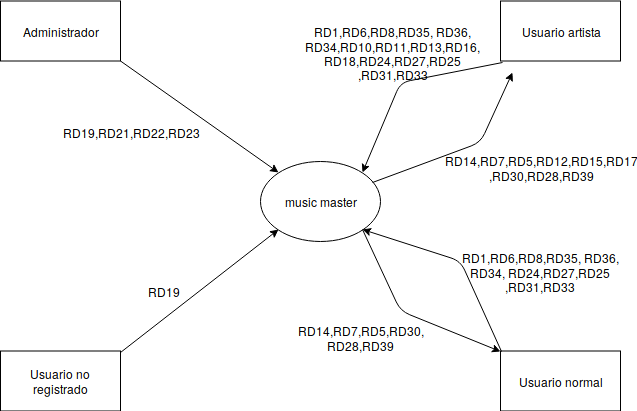
\includegraphics[width=0.6\textwidth]{imagenes/caja_negra.png}\par\vspace{1cm}}
  \end{center}
\subsection{Esquema armazón DFD0.}
  \begin{center}
  \shadowbox{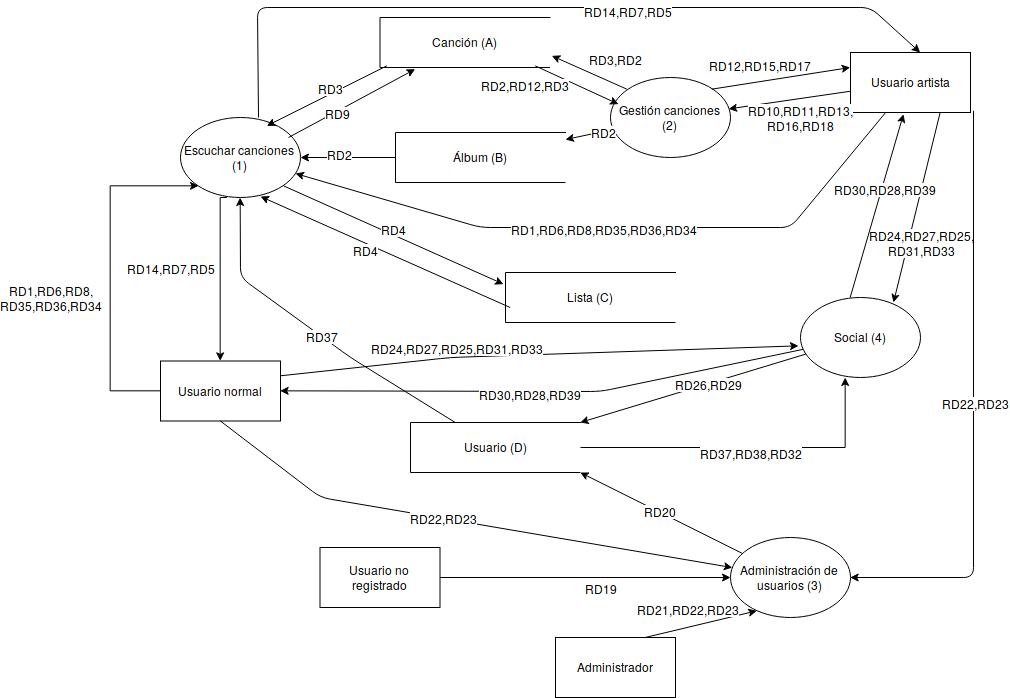
\includegraphics[width=0.6\textwidth]{imagenes/DFD0.png}\par\vspace{1cm}}
  \end{center}
\subsection{Esquemas externos del DFD0.}
	%No se que esquemas son estos
\subsection{Esquema armazón D (ER0).}
	Unión de los esquemas externos.
	%No se que esquema es este	
\subsection{Refinamientos.}
\subsubsection{Módulo social.}
\paragraph{DFD1}
\begin{center}
\shadowbox{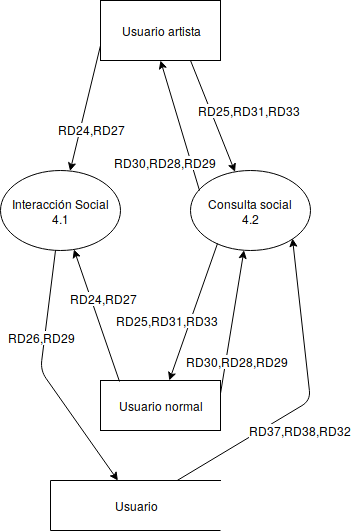
\includegraphics[width=0.6\textwidth]{imagenes/DFD1_social.png}\par\vspace{1cm}}
\end{center}	
\paragraph{DFD2}
\subparagraph{Primer plano de refinamiento.}
\begin{center}
\shadowbox{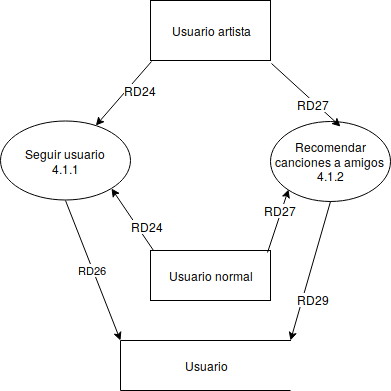
\includegraphics[width=0.6\textwidth]{imagenes/DFD2_4-1_social.png}\par\vspace{1cm}}    
\end{center}
\newpage
\subparagraph{Segundo plano de refinamiento.}
\begin{center}
\shadowbox{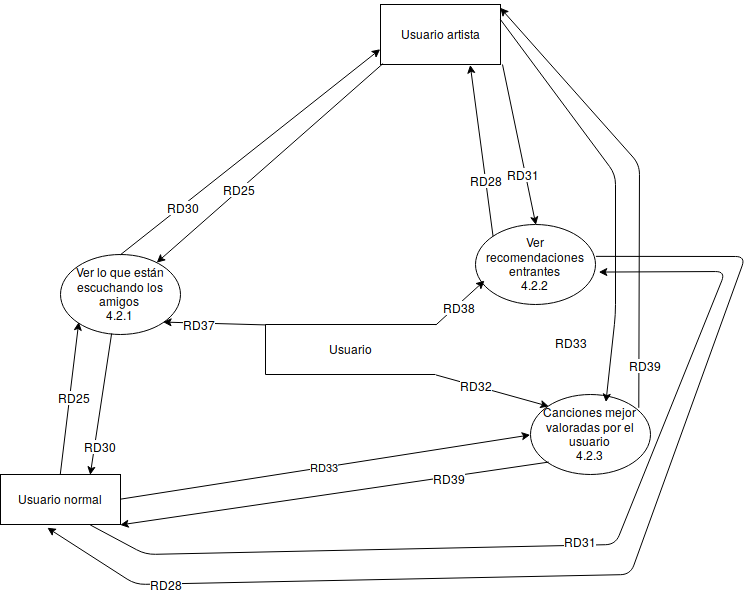
\includegraphics[width=0.6\textwidth]{imagenes/DFD2_4-2_social.png}\par\vspace{1cm}}    
\end{center}
\paragraph{Esquema externo.}
\begin{center}
\shadowbox{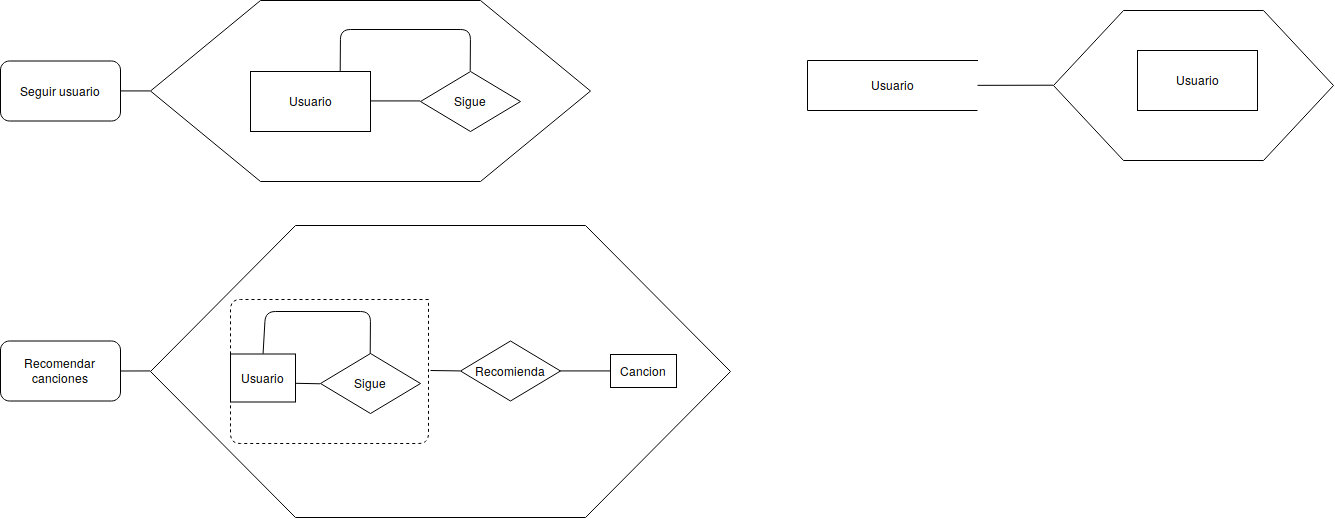
\includegraphics[width=1.0\textwidth]{imagenes/EE_social.png}\par\vspace{1cm}}
\end{center} 
\subsubsection{Módulo escuchar canciones.}
\subsubsection{Unión de módulos DFD1.}
\begin{center}
\shadowbox{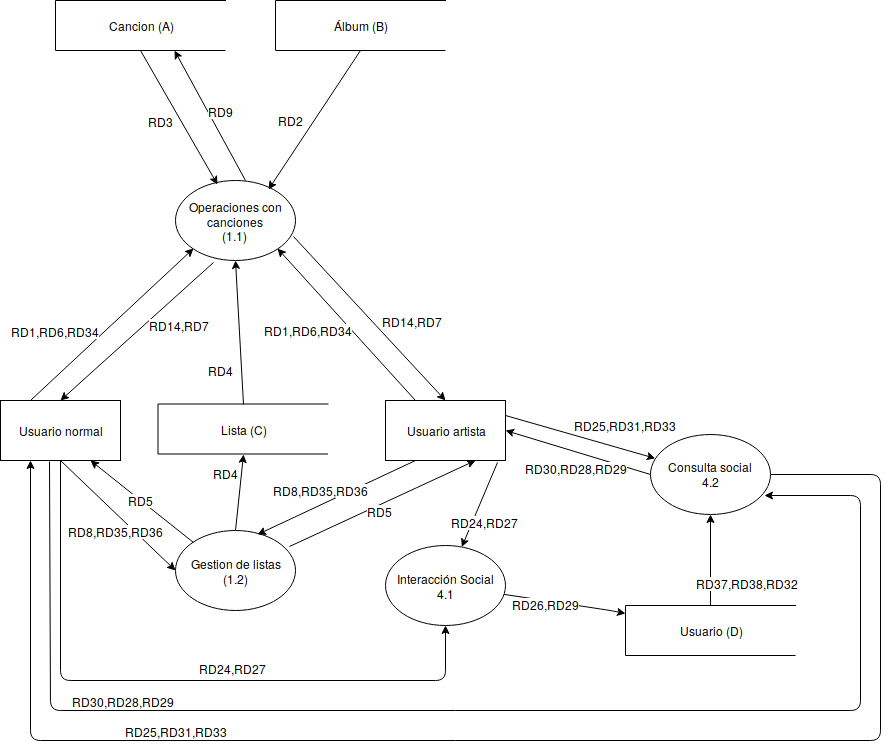
\includegraphics[width=0.7\textwidth]{imagenes/DFD1_union.png}\par\vspace{1cm}}
\end{center}
\subsubsection{Unión de módulos DFD2.}
\begin{center}
\shadowbox{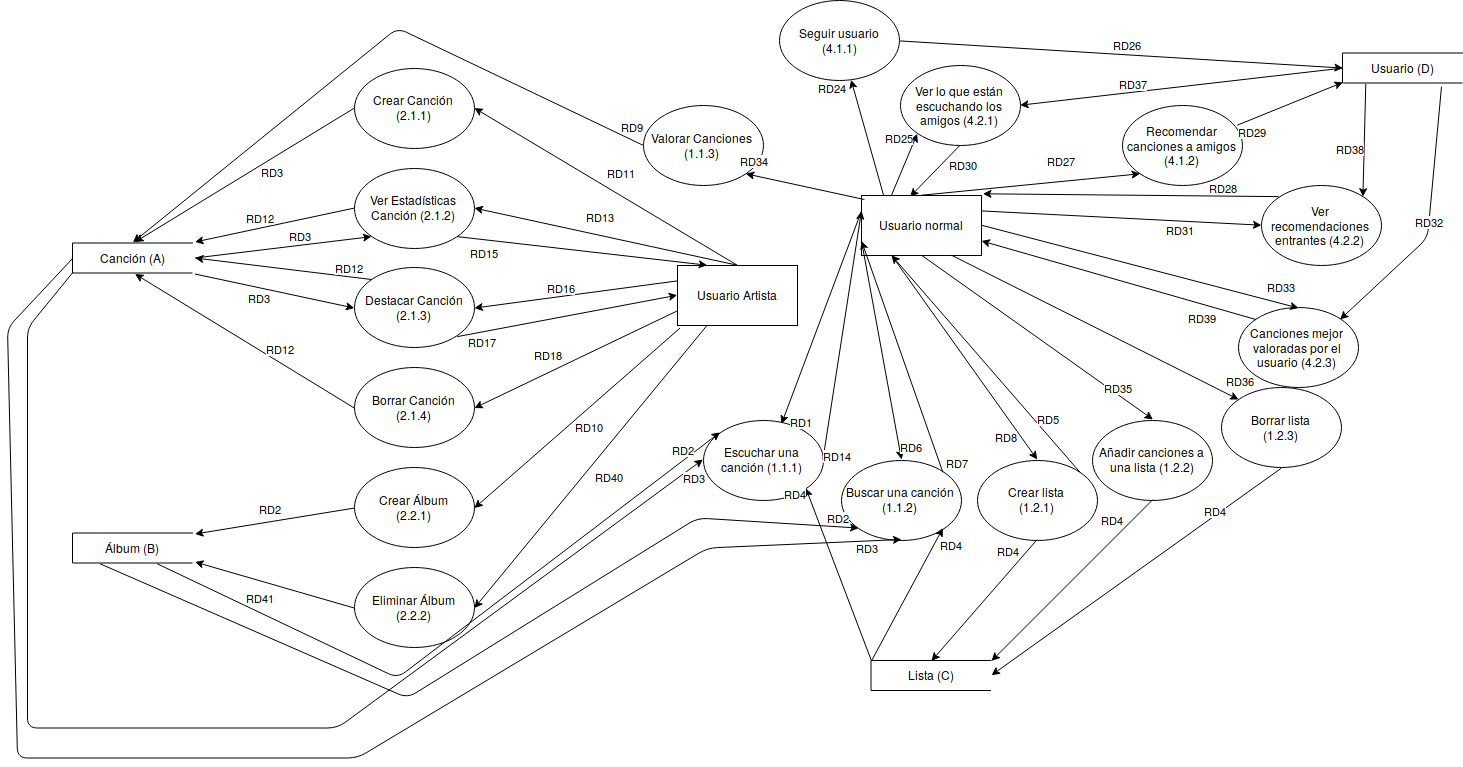
\includegraphics[width=1.0\textwidth]{imagenes/DFD2_union.png}\par\vspace{1cm}}
\end{center}

\subsection{Esquema entidad relación.}
\begin{center}
\shadowbox{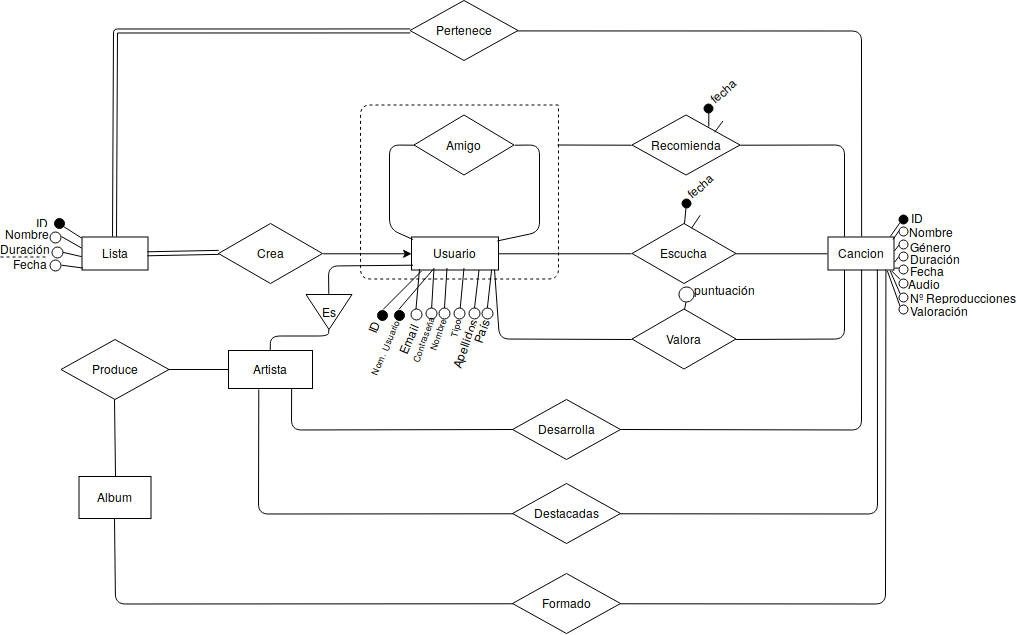
\includegraphics[width=1.0\textwidth]{imagenes/ER.png}\par\vspace{1cm}}
\end{center}

\subsection{Paso a tablas.}
Tabla usuario.

	Clave primaria: ID usuario.
	
	Resto de atributos: nombre usuario, nombre artistico, email, contraseña, nombre, apellidos, tipo, pais.

Tabla canción.

	Clave primaria: ID cancion.
	
	Resto de atributos: nombre, genero, duración, fecha, ruta audio, numero de reproducciones, valoración.


Tabla lista.

	Clave primaria: ID lista.
	
	Resto de atributos: nombre, fecha, duración.
	
Tabla amigo.

	Clave primaria: ID usuario1, ID usuario2.
	Ambas como claves externas a ID usuario de la tabla usuario.
	
Tabla recomienda.

	Clave primaria: ID usuario1, ID usuario2, ID cancion, fecha.
	
	ID usuario1 e ID usuario2 como claves externas a la tabla amigo.
	ID cancion como clave externa a la tabla cancion.
	
Tabla escucha.
	
	Clave primaria: ID usuario1, ID usuario2, fecha.
	
	ID usuario1 e ID usuario2 como claves externas a la tabla cancion.
	
Tabla valora.

	Clave primaria: ID usuario, ID cancion.
	
	ID usuario como clave externa a la tabla usuario.
	ID cancion como clave externa a la tabla cancion.
	
	Resto de atributos: puntuación.
	
Tabla pertenece.

	Clave primaria: ID lista, ID cancion.
	
	ID lista como clave externa a la tabla lista.
	ID cancion como clave externa a la tabla cancion.
	
Tabla crea.
	
	Clave primaria: ID lista, ID usuario.
	
	ID lista como clave externa a la tabla lista.
	ID usuario como clave externa la tabla usuario.
	
\section{Implementación.}
\subsection{Diseño físico de la base de datos.}
\newpage

\subsubsection{Sentencias SQL.}
\begin{lstlisting}[language=SQL]
create table usuario(
    id_usuario char(8) constraint id_usuario_no_nulo not null
    constraint id_usuario_primaria primary key,
    nombre_usuario varchar2(15) 
    	constraint nombre_usuario_no_nulo not null
    constraint nombre_usuario_candidata unique,
    email_u varchar2(40) constraint email_no_nulo not null,
    contrasenia_u varchar2(40) constraint contrasenia_no_nula not null,
    nombre_per varchar2(15) constraint nombre_no_nulo not null,
    apellidos_per varchar2(30),
    tipo varchar2(7) constraint tipo_correcto 
    	check (tipo in ('artista','usuario')),
    pais varchar2(20),
    nombre_artistico varchar2(50));
    
create table cancion(
    id_cancion char(8) constraint id_cancion_no_nulo not null
    constraint id_cancion_primaria primary key,
    nombre_cancion varchar2(50) 
    	constraint nombre_cancion_no_nulo not null,
    genero varchar2(20) constraint genero_no_nulo not null,
    duracion_seg number(3) constraint duracion_seg_no_nula not null,
    fecha_c date constraint fecha_cancion_no_nula not null,
    ruta_audio varchar2(100),
    num_repro number(10),
    valoracion number(1,2));
    
create table lista(
    id_lista char(8) constraint id_lista_no_nulo not null
    constraint id_lista_primaria primary key,
    nombre_lista varchar2(50) constraint nombre_lista_no_nulo not null,
    fecha_l date constraint fecha_lista_no_nula not null,
    duracion_seg number(6));
\end{lstlisting}
\newpage
\begin{lstlisting}[language=SQL]
create table pertenece(
    id_lista,
    id_cancion,
    constraint pertenece_clave_primaria primary key (id_lista,id_cancion),
    constraint id_lista_ext_pertenece foreign key(id_lista) 
    	references lista(id_lista),
    constraint id_cancion_ext_pertenece foreign key(id_cancion) 
    	references cancion(id_cancion));

create table crea(
    id_usuario,
    id_lista,
    constraint crea_clave_primaria primary key (id_usuario,id_lista),
    constraint id_usuario_ext_crea foreign key(id_usuario) 
    	references usuario(id_usuario),
    constraint id_lista_ext_crea foreign key(id_lista) 
    	references lista(id_lista));

CREATE TABLE amigo
  (
    id_usuario1,
    id_usuario2,
    CONSTRAINT clave_primaria PRIMARY KEY (id_usuario1,id_usuario2),
    CONSTRAINT id_usuario1_ext_pertenece FOREIGN KEY(id_usuario1) 
    REFERENCES usuario(id_usuario),
    CONSTRAINT id_usuario2_ext_pertenece FOREIGN KEY(id_usuario2) 
    REFERENCES usuario(id_usuario)
  );
  
create table recomienda(
  id_usuario1,
  id_usuario2,
  id_cancion,
  fecha date not null,
  constraint clave_pri 
  	primary key (id_usuario1,id_usuario2,id_cancion,fecha),
  foreign key (id_usuario1,id_usuario2) 
  	references amigo(id_usuario1,id_usuario2),
  foreign key (id_cancion) references cancion(id_cancion)
);
\end{lstlisting}
\newpage
\begin{lstlisting}[language=SQL]
create table valora(
  id_usuario,
  id_cancion,
  puntuacion number(1,1),
  primary key (id_usuario,id_cancion),
  foreign key (id_usuario) references usuario(id_usuario),
  foreign key (id_cancion) references cancion(id_cancion)
);

create table escucha(
  id_usuario,
  id_cancion,
  fecha date not null,
  primary key (id_usuario,id_cancion,fecha),
  foreign key (id_usuario) references usuario(id_usuario),
  foreign key (id_cancion) references cancion(id_cancion)
);

\end{lstlisting}
\newpage
\subsection{Implementación modulo social.}
\subsubsection{Implementación del disparador.}
	Este disparador controla la inserción de una tupla en la tabla recomendación. Es decir comprueba una condición cuando un usuario recomienda una canción a otro usuario. Dicha condición consiste en que un usuario no puede recomendar una canción si no la ha escuchado previamente.
	
	Básicamente, el funcionamiento consiste en comprobar la tabla escucha (donde reside el registro de reproducciones que han realizado los usuarios) y mirar si el usuario que recomienda ha reproducido la canción que se recomienda canción. Si no encuentra ningún resultado, levanta una excepción.

\begin{lstlisting}[language=SQL]
create or replace TRIGGER dario_trigg
BEFORE INSERT ON recomienda
FOR EACH ROW
DECLARE
no_escuchada EXCEPTION;
existe number;
BEGIN
SELECT count(*) INTO existe FROM escucha 
WHERE id_cancion = :new.id_cancion and id_usuario = :new.id_usuario1;
    IF (existe = 0) THEN
           RAISE no_escuchada;
    END IF;
    EXCEPTION
    WHEN no_escuchada THEN
    RAISE_APPLICATION_ERROR(-20000,'No has escuchado la cancion');
END;
\end{lstlisting}
\newpage
\subsubsection{Implementación de un proceso.}
	El proceso acordado para la implementación consiste mostrar que están escuchando mis amigos. Debido a la dificultad de mostrar lo que se está reproduciendo en un instante, se decidió mostrar las reproducciones realizadas ``hoy'', es decir, en un día completo.
	
	El proceso ha sido implementado en Python y la interfaz es línea de comandos (CLI), debido a la falta de tiempo y el poco conocimiento a cerca de interfaces gráficas. 
	
	La conexión a la base de datos se realiza mediante el paquete ``cx\_Oracle'', que nos permite realizar las consultas y manejar los datos consultados.



\begin{lstlisting}[language=Python,frame=single,showstringspaces=false]
#!/usr/bin/python
# -*- coding: utf-8 -*-
import os
import cx_Oracle


def menu():
	print ("Opciones disponibles:")
	print ("\t1 - Ver que han escuchado mis amigos hoy.")
	print ("\t0 - Salir")

def mostrar_info_amigo(info_amigo):
	for row in info_amigo:
		print "Usuario: " + row[0]
		print "Nombre: " + row[1] + " " + row[2]
	print "-----------------------------------------"

###########################################################

conn_str = 'USUARIO/PASSWORD@HOSTNAME:PORT/SERVICENAME'
conn = cx_Oracle.connect(conn_str)

my_id = 'UN000002' # Hipotético usuario logueado en el sistema
hoy = '17/09/2017' # Hipotécica fecha actual
\end{lstlisting}
\newpage
\begin{lstlisting}[language=Python,frame=single,tabsize=2,showstringspaces=false]
c = conn.cursor()

while True:
	menu()

	opcionMenu = str(input("Selecciona una acción: "))

	if opcionMenu == '1':
	#Listamos los amigos
		c.execute("SELECT id_usuario2 FROM amigo 
						      WHERE id_usuario1 = '%s'" % (my_id))
		id_amigos = c.fetchall()
		
		contador = 1
		info_amigo = []
		#MOSTRAR LISTA DE AMIGOS
		print "-----------------------------------------"
		for ID in id_amigos: 
			c.execute("SELECT nombre_usuario, nombre_per, apellidos_per 
			              FROM usuario WHERE id_usuario = '%s'" % (ID))
			info_amigo = c.fetchall()
			print "Amigo " + str(contador)
			mostrar_info_amigo(info_amigo)
			contador += 1

		opcionMenu = str(input("Selecciona un amigo: "))
		num_usuario = int(opcionMenu)-1

		#RECUPERAR ID AMIGO SELECCIONADO
		c.execute("SELECT id_usuario2 FROM amigo 
		               WHERE id_usuario1 = '%s'" % (my_id))
		id_amigos = c.fetchall()
		amigo = id_amigos[num_usuario]
\end{lstlisting}
\newpage
\begin{lstlisting}[language=Python,frame=single,tabsize=2,showstringspaces=false]
		#Recuperamos nombre de amigo
		c.execute("SELECT nombre_usuario FROM usuario 
		               WHERE id_usuario = '%s'" % (amigo[0]))
		nombre_amigo = c.fetchone()
		
		#Consultamos las canciones escuchadas hoy por el amigo 
		#seleccionado
		c.execute("SELECT * FROM escucha WHERE id_usuario = '%s' 
				and fecha = to_date('%s','DD/MM/YYYY')" % (amigo[0], hoy))
		canciones = c.fetchall()


		#Mostramos lista de canciones escuchadas por el amigo 
		#seleccionado
		print "\n-----------------------------------------"				
		print "Lista de canciones escuchadas hoy por %s:" 
		                                              % (nombre_amigo)
		for cancion in canciones:
			c.execute("SELECT nombre_cancion FROM cancion 
			          WHERE id_cancion = '%s'" % (cancion[1]))
			nombre_cancion = c.fetchone()[0]
			print "- " + nombre_cancion

		print "\n\n"
	

	if opcionMenu == '0':
		conn.close()
		break
\end{lstlisting}

\end{document}
